\documentclass[1p]{elsarticle_modified}
%\bibliographystyle{elsarticle-num}

%\usepackage[colorlinks]{hyperref}
%\usepackage{abbrmath_seonhwa} %\Abb, \Ascr, \Acal ,\Abf, \Afrak
\usepackage{amsfonts}
\usepackage{amssymb}
\usepackage{amsmath}
\usepackage{amsthm}
\usepackage{scalefnt}
\usepackage{amsbsy}
\usepackage{kotex}
\usepackage{caption}
\usepackage{subfig}
\usepackage{color}
\usepackage{graphicx}
\usepackage{xcolor} %% white, black, red, green, blue, cyan, magenta, yellow
\usepackage{float}
\usepackage{setspace}
\usepackage{hyperref}

\usepackage{tikz}
\usetikzlibrary{arrows}

\usepackage{multirow}
\usepackage{array} % fixed length table
\usepackage{hhline}

%%%%%%%%%%%%%%%%%%%%%
\makeatletter
\renewcommand*\env@matrix[1][\arraystretch]{%
	\edef\arraystretch{#1}%
	\hskip -\arraycolsep
	\let\@ifnextchar\new@ifnextchar
	\array{*\c@MaxMatrixCols c}}
\makeatother %https://tex.stackexchange.com/questions/14071/how-can-i-increase-the-line-spacing-in-a-matrix
%%%%%%%%%%%%%%%

\usepackage[normalem]{ulem}

\newcommand{\msout}[1]{\ifmmode\text{\sout{\ensuremath{#1}}}\else\sout{#1}\fi}
%SOURCE: \msout is \stkout macro in https://tex.stackexchange.com/questions/20609/strikeout-in-math-mode

\newcommand{\cancel}[1]{
	\ifmmode
	{\color{red}\msout{#1}}
	\else
	{\color{red}\sout{#1}}
	\fi
}

\newcommand{\add}[1]{
	{\color{blue}\uwave{#1}}
}

\newcommand{\replace}[2]{
	\ifmmode
	{\color{red}\msout{#1}}{\color{blue}\uwave{#2}}
	\else
	{\color{red}\sout{#1}}{\color{blue}\uwave{#2}}
	\fi
}

\newcommand{\Sol}{\mathcal{S}} %segment
\newcommand{\D}{D} %diagram
\newcommand{\A}{\mathcal{A}} %arc


%%%%%%%%%%%%%%%%%%%%%%%%%%%%%5 test

\def\sl{\operatorname{\textup{SL}}(2,\Cbb)}
\def\psl{\operatorname{\textup{PSL}}(2,\Cbb)}
\def\quan{\mkern 1mu \triangleright \mkern 1mu}

\theoremstyle{definition}
\newtheorem{thm}{Theorem}[section]
\newtheorem{prop}[thm]{Proposition}
\newtheorem{lem}[thm]{Lemma}
\newtheorem{ques}[thm]{Question}
\newtheorem{cor}[thm]{Corollary}
\newtheorem{defn}[thm]{Definition}
\newtheorem{exam}[thm]{Example}
\newtheorem{rmk}[thm]{Remark}
\newtheorem{alg}[thm]{Algorithm}

\newcommand{\I}{\sqrt{-1}}
\begin{document}

%\begin{frontmatter}
%
%\title{Boundary parabolic representations of knots up to 8 crossings}
%
%%% Group authors per affiliation:
%\author{Yunhi Cho} 
%\address{Department of Mathematics, University of Seoul, Seoul, Korea}
%\ead{yhcho@uos.ac.kr}
%
%
%\author{Seonhwa Kim} %\fnref{s_kim}}
%\address{Center for Geometry and Physics, Institute for Basic Science, Pohang, 37673, Korea}
%\ead{ryeona17@ibs.re.kr}
%
%\author{Hyuk Kim}
%\address{Department of Mathematical Sciences, Seoul National University, Seoul 08826, Korea}
%\ead{hyukkim@snu.ac.kr}
%
%\author{Seokbeom Yoon}
%\address{Department of Mathematical Sciences, Seoul National University, Seoul, 08826,  Korea}
%\ead{sbyoon15@snu.ac.kr}
%
%\begin{abstract}
%We find all boundary parabolic representation of knots up to 8 crossings.
%
%\end{abstract}
%\begin{keyword}
%    \MSC[2010] 57M25 
%\end{keyword}
%
%\end{frontmatter}

%\linenumbers
%\tableofcontents
%
\newcommand\colored[1]{\textcolor{white}{\rule[-0.35ex]{0.8em}{1.4ex}}\kern-0.8em\color{red} #1}%
%\newcommand\colored[1]{\textcolor{white}{ #1}\kern-2.17ex	\textcolor{white}{ #1}\kern-1.81ex	\textcolor{white}{ #1}\kern-2.15ex\color{red}#1	}

{\Large $\underline{10_{163}~(K10n_{35})}$}

\setlength{\tabcolsep}{10pt}
\renewcommand{\arraystretch}{1.6}
\vspace{1cm}\begin{tabular}{m{100pt}>{\centering\arraybackslash}m{274pt}}
\multirow{5}{120pt}{
	\centering
	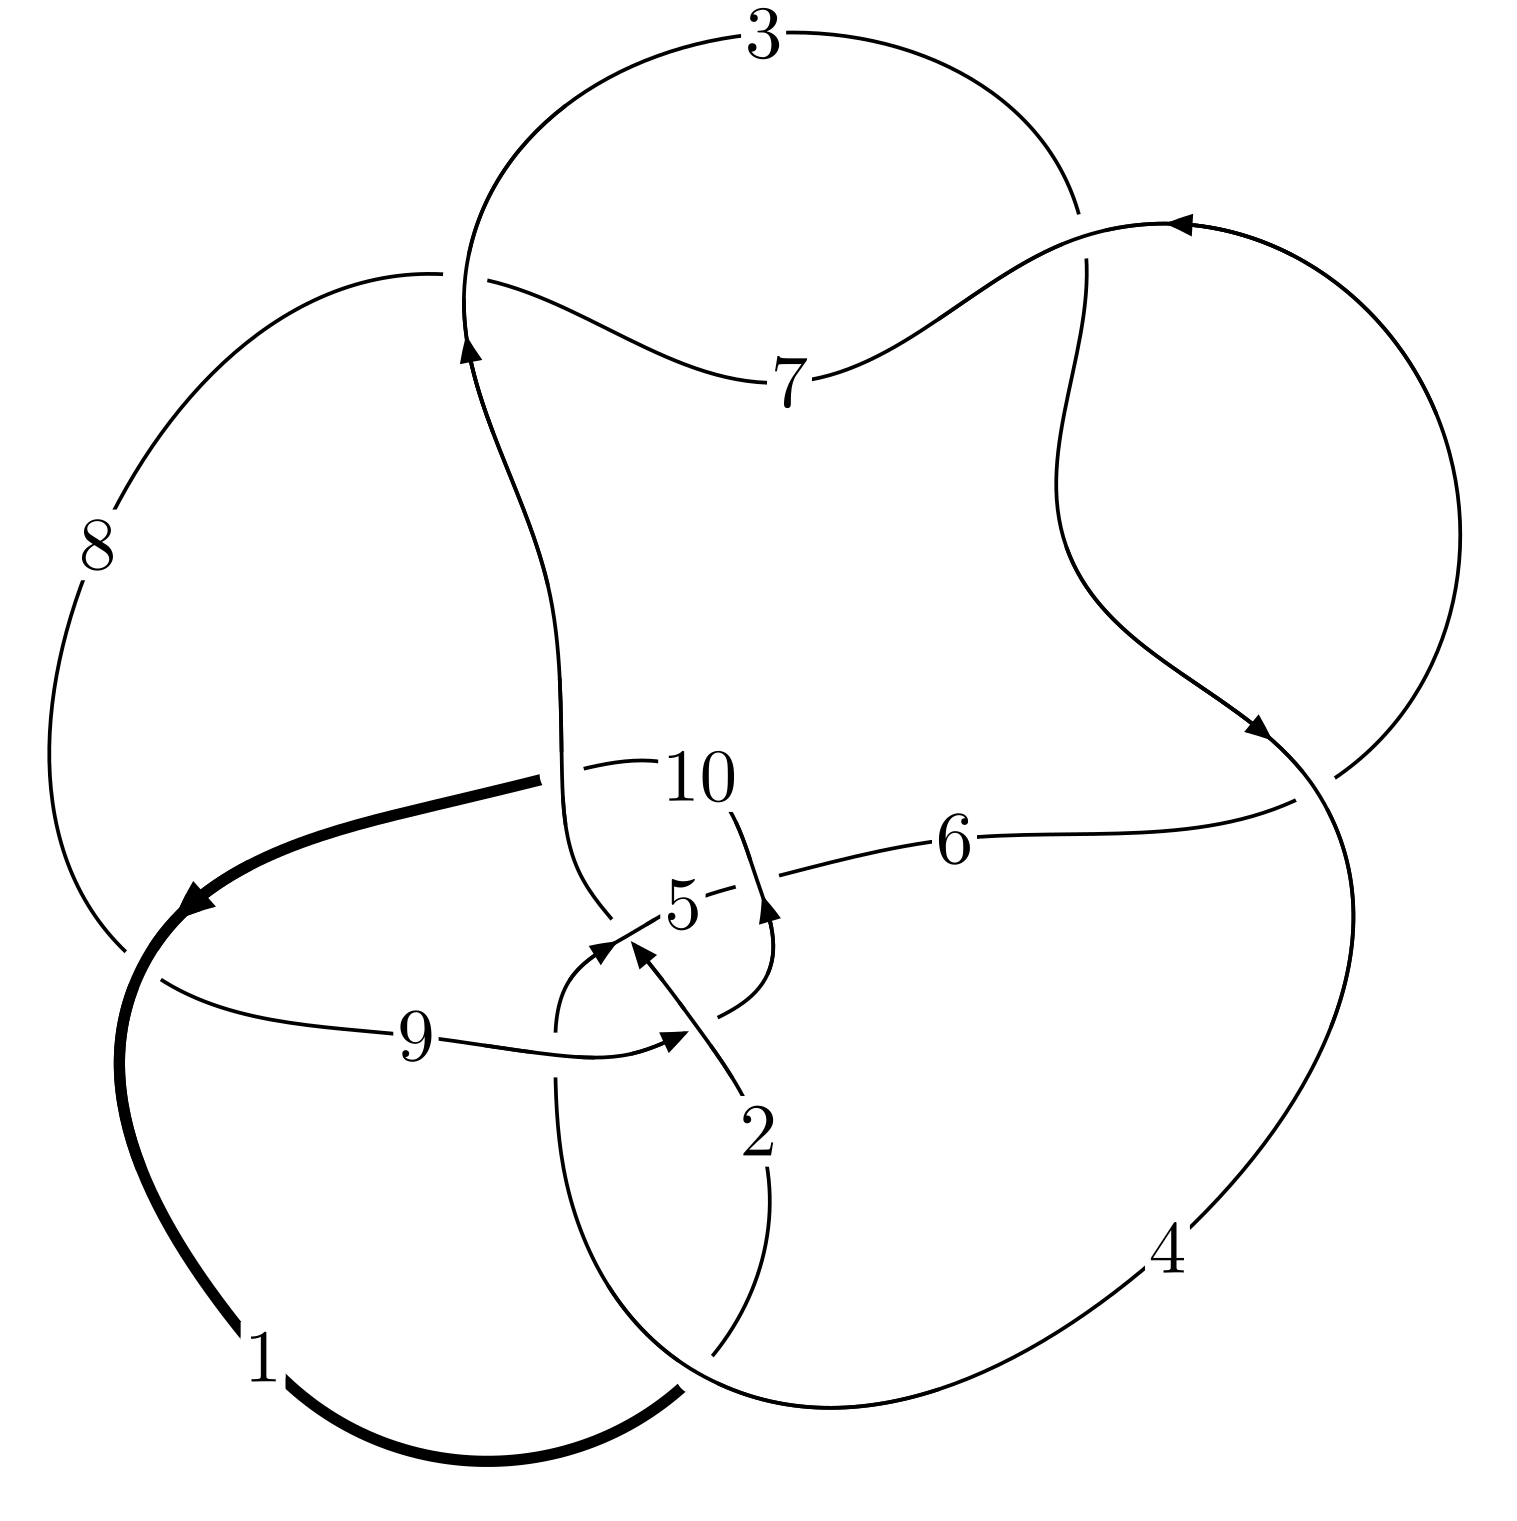
\includegraphics[width=112pt]{../../../GIT/diagram.site/Diagrams/png/247_10_163.png}\\
\ \ \ A knot diagram\footnotemark}&
\allowdisplaybreaks
\textbf{Linearized knot diagam} \\
\cline{2-2}
 &
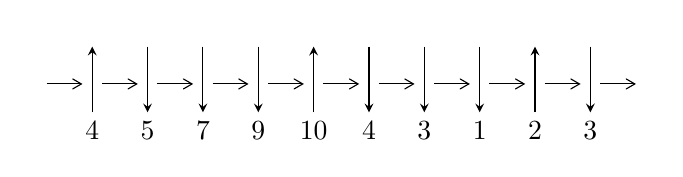
\begin{tikzpicture}[x=20pt, y=17pt]
	% nodes
	\node (C0) at (0, 0) {};
	\node (C1) at (1, 0) {};
	\node (C1U) at (1, +1) {};
	\node (C1D) at (1, -1) {4};

	\node (C2) at (2, 0) {};
	\node (C2U) at (2, +1) {};
	\node (C2D) at (2, -1) {5};

	\node (C3) at (3, 0) {};
	\node (C3U) at (3, +1) {};
	\node (C3D) at (3, -1) {7};

	\node (C4) at (4, 0) {};
	\node (C4U) at (4, +1) {};
	\node (C4D) at (4, -1) {9};

	\node (C5) at (5, 0) {};
	\node (C5U) at (5, +1) {};
	\node (C5D) at (5, -1) {10};

	\node (C6) at (6, 0) {};
	\node (C6U) at (6, +1) {};
	\node (C6D) at (6, -1) {4};

	\node (C7) at (7, 0) {};
	\node (C7U) at (7, +1) {};
	\node (C7D) at (7, -1) {3};

	\node (C8) at (8, 0) {};
	\node (C8U) at (8, +1) {};
	\node (C8D) at (8, -1) {1};

	\node (C9) at (9, 0) {};
	\node (C9U) at (9, +1) {};
	\node (C9D) at (9, -1) {2};

	\node (C10) at (10, 0) {};
	\node (C10U) at (10, +1) {};
	\node (C10D) at (10, -1) {3};
	\node (C11) at (11, 0) {};

	% arrows
	\draw[->,>={angle 60}]
	(C0) edge (C1) (C1) edge (C2) (C2) edge (C3) (C3) edge (C4) (C4) edge (C5) (C5) edge (C6) (C6) edge (C7) (C7) edge (C8) (C8) edge (C9) (C9) edge (C10) (C10) edge (C11) ;	\draw[->,>=stealth]
	(C1D) edge (C1U) (C2U) edge (C2D) (C3U) edge (C3D) (C4U) edge (C4D) (C5D) edge (C5U) (C6U) edge (C6D) (C7U) edge (C7D) (C8U) edge (C8D) (C9D) edge (C9U) (C10U) edge (C10D) ;
	\end{tikzpicture} \\
\hhline{~~} \\& 
\textbf{Solving Sequence} \\ \cline{2-2} 
 &
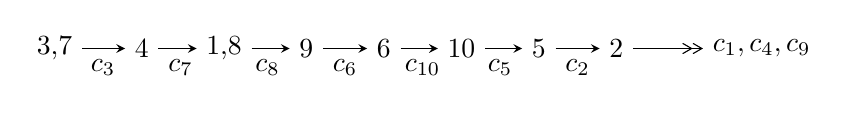
\begin{tikzpicture}[x=28pt, y=7pt]
	% node
	\node (A0) at (-1/8, 0) {3,7};
	\node (A1) at (1, 0) {4};
	\node (A2) at (33/16, 0) {1,8};
	\node (A3) at (25/8, 0) {9};
	\node (A4) at (33/8, 0) {6};
	\node (A5) at (41/8, 0) {10};
	\node (A6) at (49/8, 0) {5};
	\node (A7) at (57/8, 0) {2};
	\node (C1) at (1/2, -1) {$c_{3}$};
	\node (C2) at (3/2, -1) {$c_{7}$};
	\node (C3) at (21/8, -1) {$c_{8}$};
	\node (C4) at (29/8, -1) {$c_{6}$};
	\node (C5) at (37/8, -1) {$c_{10}$};
	\node (C6) at (45/8, -1) {$c_{5}$};
	\node (C7) at (53/8, -1) {$c_{2}$};
	\node (A8) at (9, 0) {$c_{1},c_{4},c_{9}$};

	% edge
	\draw[->,>=stealth]	
	(A0) edge (A1) (A1) edge (A2) (A2) edge (A3) (A3) edge (A4) (A4) edge (A5) (A5) edge (A6) (A6) edge (A7) ;
	\draw[->>,>={angle 60}]	
	(A7) edge (A8);
\end{tikzpicture} \\ 

\end{tabular} \\

\footnotetext{
The image of knot diagram is generated by the software ``\textbf{Draw programme}" developed by Andrew Bartholomew(\url{http://www.layer8.co.uk/maths/draw/index.htm\#Running-draw}), where we modified some parts for our purpose(\url{https://github.com/CATsTAILs/LinksPainter}).
}\phantom \\ \newline 
\centering \textbf{Ideals for irreducible components\footnotemark of $X_{\text{par}}$} 
 
\begin{align*}
I^u_{1}&=\langle 
u^{13}+5 u^{12}+15 u^{11}+31 u^{10}+50 u^9+63 u^8+61 u^7+42 u^6+17 u^5+u^4-8 u^3-9 u^2+b-8 u+1,\\
\phantom{I^u_{1}}&\phantom{= \langle  }-4 u^{13}-25 u^{12}+\cdots+5 a+36,\\
\phantom{I^u_{1}}&\phantom{= \langle  }u^{14}+5 u^{13}+15 u^{12}+30 u^{11}+47 u^{10}+55 u^9+48 u^8+22 u^7-2 u^6-17 u^5-15 u^4-14 u^3-4 u^2+u+5\rangle \\
I^u_{2}&=\langle 
- u^3 a- u^3- a u+3 u^2+3 b+a-4 u+1,\;u^3 a- u^2 a+2 u^3+a^2-3 u^2+2 a+2 u+3,\;u^4- u^3+u^2+u+1\rangle \\
I^u_{3}&=\langle 
- u^5+2 u^4-4 u^3+4 u^2+b-3 u+1,\;- u^4+2 u^3-4 u^2+a+3 u-3,\;u^6-2 u^5+4 u^4-4 u^3+4 u^2- u+1\rangle \\
I^u_{4}&=\langle 
- u^3 a+u^2 a- a u+b+a+u-1,\;- u^3 a+3 u^2 a+a^2-3 a u- u^2+u,\;u^4-2 u^3+2 u^2- u+1\rangle \\
\\
I^v_{1}&=\langle 
a,\;b+1,\;v-1\rangle \\
\end{align*}
\raggedright * 5 irreducible components of $\dim_{\mathbb{C}}=0$, with total 37 representations.\\
\footnotetext{All coefficients of polynomials are rational numbers. But the coefficients are sometimes approximated in decimal forms when there is not enough margin.}
\newpage
\renewcommand{\arraystretch}{1}
\centering \section*{I. $I^u_{1}= \langle u^{13}+5 u^{12}+\cdots+b+1,\;-4 u^{13}-25 u^{12}+\cdots+5 a+36,\;u^{14}+5 u^{13}+\cdots+u+5 \rangle$}
\flushleft \textbf{(i) Arc colorings}\\
\begin{tabular}{m{7pt} m{180pt} m{7pt} m{180pt} }
\flushright $a_{3}=$&$\begin{pmatrix}1\\0\end{pmatrix}$ \\
\flushright $a_{7}=$&$\begin{pmatrix}0\\u\end{pmatrix}$ \\
\flushright $a_{4}=$&$\begin{pmatrix}1\\u^2\end{pmatrix}$ \\
\flushright $a_{1}=$&$\begin{pmatrix}\frac{4}{5} u^{13}+5 u^{12}+\cdots-\frac{81}{5} u-\frac{36}{5}\\- u^{13}-5 u^{12}+\cdots+8 u-1\end{pmatrix}$ \\
\flushright $a_{8}=$&$\begin{pmatrix}- u\\u\end{pmatrix}$ \\
\flushright $a_{9}=$&$\begin{pmatrix}\frac{11}{5} u^{13}+8 u^{12}+\cdots+\frac{61}{5} u+\frac{51}{5}\\- u^{13}- u^{12}+\cdots-14 u+6\end{pmatrix}$ \\
\flushright $a_{6}=$&$\begin{pmatrix}u\\u^3+u\end{pmatrix}$ \\
\flushright $a_{10}=$&$\begin{pmatrix}-\frac{1}{5} u^{13}+2 u^{11}+\cdots-\frac{41}{5} u-\frac{41}{5}\\- u^{13}-5 u^{12}+\cdots+8 u-1\end{pmatrix}$ \\
\flushright $a_{5}=$&$\begin{pmatrix}-\frac{9}{5} u^{13}-8 u^{12}+\cdots+\frac{36}{5} u+\frac{26}{5}\\- u^{13}-4 u^{12}+\cdots-6 u-9\end{pmatrix}$ \\
\flushright $a_{2}=$&$\begin{pmatrix}-\frac{1}{5} u^{13}- u^{12}+\cdots-\frac{16}{5} u-\frac{16}{5}\\-2 u^{12}-9 u^{11}+\cdots+14 u+4\end{pmatrix}$\\&\end{tabular}
\flushleft \textbf{(ii) Obstruction class $= -1$}\\~\\
\flushleft \textbf{(iii) Cusp Shapes $= -4 u^{13}-5 u^{12}+2 u^{11}+43 u^{10}+98 u^9+192 u^8+233 u^7+231 u^6+106 u^5+55 u^4-27 u^3-21 u^2-60 u-6$}\\~\\
\newpage\renewcommand{\arraystretch}{1}
\flushleft \textbf{(iv) u-Polynomials at the component}\newline \\
\begin{tabular}{m{50pt}|m{274pt}}
Crossings & \hspace{64pt}u-Polynomials at each crossing \\
\hline $$\begin{aligned}c_{1},c_{5}\end{aligned}$$&$\begin{aligned}
&u^{14}+4 u^{12}+\cdots-2 u+3
\end{aligned}$\\
\hline $$\begin{aligned}c_{2},c_{4}\end{aligned}$$&$\begin{aligned}
&u^{14}- u^{13}+\cdots-3 u+1
\end{aligned}$\\
\hline $$\begin{aligned}c_{3},c_{6},c_{7}\end{aligned}$$&$\begin{aligned}
&u^{14}-5 u^{13}+\cdots- u+5
\end{aligned}$\\
\hline $$\begin{aligned}c_{8},c_{10}\end{aligned}$$&$\begin{aligned}
&u^{14}-10 u^{12}+\cdots-2 u+1
\end{aligned}$\\
\hline $$\begin{aligned}c_{9}\end{aligned}$$&$\begin{aligned}
&u^{14}+10 u^{13}+\cdots+28 u+5
\end{aligned}$\\
\hline
\end{tabular}\\~\\
\newpage\renewcommand{\arraystretch}{1}
\flushleft \textbf{(v) Riley Polynomials at the component}\newline \\
\begin{tabular}{m{50pt}|m{274pt}}
Crossings & \hspace{64pt}Riley Polynomials at each crossing \\
\hline $$\begin{aligned}c_{1},c_{5}\end{aligned}$$&$\begin{aligned}
&y^{14}+8 y^{13}+\cdots+62 y+9
\end{aligned}$\\
\hline $$\begin{aligned}c_{2},c_{4}\end{aligned}$$&$\begin{aligned}
&y^{14}-5 y^{13}+\cdots-13 y+1
\end{aligned}$\\
\hline $$\begin{aligned}c_{3},c_{6},c_{7}\end{aligned}$$&$\begin{aligned}
&y^{14}+5 y^{13}+\cdots-41 y+25
\end{aligned}$\\
\hline $$\begin{aligned}c_{8},c_{10}\end{aligned}$$&$\begin{aligned}
&y^{14}-20 y^{13}+\cdots-6 y+1
\end{aligned}$\\
\hline $$\begin{aligned}c_{9}\end{aligned}$$&$\begin{aligned}
&y^{14}+26 y^{12}+\cdots+246 y+25
\end{aligned}$\\
\hline
\end{tabular}\\~\\
\newpage\flushleft \textbf{(vi) Complex Volumes and Cusp Shapes}
$$\begin{array}{c|c|c}  
\text{Solutions to }I^u_{1}& \I (\text{vol} + \sqrt{-1}CS) & \text{Cusp shape}\\
 \hline 
\begin{aligned}
u &= \phantom{-}0.269018 + 0.823102 I \\
a &= \phantom{-}0.699358 + 0.808665 I \\
b &= -0.020522 - 0.611730 I\end{aligned}
 & \phantom{-}0.79193 - 2.01282 I & -1.55516 + 4.15380 I \\ \hline\begin{aligned}
u &= \phantom{-}0.269018 - 0.823102 I \\
a &= \phantom{-}0.699358 - 0.808665 I \\
b &= -0.020522 + 0.611730 I\end{aligned}
 & \phantom{-}0.79193 + 2.01282 I & -1.55516 - 4.15380 I \\ \hline\begin{aligned}
u &= -0.809699 + 0.855443 I \\
a &= \phantom{-}0.263291 - 1.389210 I \\
b &= -1.74544 + 0.75171 I\end{aligned}
 & -4.94416 + 4.48113 I & -10.56248 - 7.82532 I \\ \hline\begin{aligned}
u &= -0.809699 - 0.855443 I \\
a &= \phantom{-}0.263291 + 1.389210 I \\
b &= -1.74544 - 0.75171 I\end{aligned}
 & -4.94416 - 4.48113 I & -10.56248 + 7.82532 I \\ \hline\begin{aligned}
u &= -0.752287 + 0.954057 I \\
a &= \phantom{-}0.894691 - 1.015850 I \\
b &= -1.66410 - 0.12170 I\end{aligned}
 & -4.62410 + 1.43381 I & -9.01327 + 1.28996 I \\ \hline\begin{aligned}
u &= -0.752287 - 0.954057 I \\
a &= \phantom{-}0.894691 + 1.015850 I \\
b &= -1.66410 + 0.12170 I\end{aligned}
 & -4.62410 - 1.43381 I & -9.01327 - 1.28996 I \\ \hline\begin{aligned}
u &= -1.104560 + 0.803929 I \\
a &= -0.696159 + 0.641405 I \\
b &= \phantom{-}1.59147 + 0.10810 I\end{aligned}
 & -6.35421 - 6.00703 I & -6.42492 + 3.68584 I \\ \hline\begin{aligned}
u &= -1.104560 - 0.803929 I \\
a &= -0.696159 - 0.641405 I \\
b &= \phantom{-}1.59147 - 0.10810 I\end{aligned}
 & -6.35421 + 6.00703 I & -6.42492 - 3.68584 I \\ \hline\begin{aligned}
u &= \phantom{-}0.633342 + 0.004347 I \\
a &= \phantom{-}0.709307 + 0.875694 I \\
b &= -0.273616 - 0.340717 I\end{aligned}
 & -1.38615 - 0.45192 I & -8.23002 + 1.56844 I \\ \hline\begin{aligned}
u &= \phantom{-}0.633342 - 0.004347 I \\
a &= \phantom{-}0.709307 - 0.875694 I \\
b &= -0.273616 + 0.340717 I\end{aligned}
 & -1.38615 + 0.45192 I & -8.23002 - 1.56844 I\\
 \hline 
 \end{array}$$\newpage$$\begin{array}{c|c|c}  
\text{Solutions to }I^u_{1}& \I (\text{vol} + \sqrt{-1}CS) & \text{Cusp shape}\\
 \hline 
\begin{aligned}
u &= \phantom{-}0.17524 + 1.43298 I \\
a &= -0.361634 + 0.364044 I \\
b &= \phantom{-}0.389777 - 0.088598 I\end{aligned}
 & \phantom{-}3.73877 - 3.84212 I & -7.98139 + 1.57763 I \\ \hline\begin{aligned}
u &= \phantom{-}0.17524 - 1.43298 I \\
a &= -0.361634 - 0.364044 I \\
b &= \phantom{-}0.389777 + 0.088598 I\end{aligned}
 & \phantom{-}3.73877 + 3.84212 I & -7.98139 - 1.57763 I \\ \hline\begin{aligned}
u &= -0.91106 + 1.12096 I \\
a &= -0.60885 + 1.30444 I \\
b &= \phantom{-}1.72243 - 0.67293 I\end{aligned}
 & -5.3164 + 13.2900 I & -4.73276 - 7.55975 I \\ \hline\begin{aligned}
u &= -0.91106 - 1.12096 I \\
a &= -0.60885 - 1.30444 I \\
b &= \phantom{-}1.72243 + 0.67293 I\end{aligned}
 & -5.3164 - 13.2900 I & -4.73276 + 7.55975 I\\
 \hline 
 \end{array}$$\newpage\newpage\renewcommand{\arraystretch}{1}
\centering \section*{II. $I^u_{2}= \langle - u^3 a- u^3- a u+3 u^2+3 b+a-4 u+1,\;u^3 a- u^2 a+2 u^3+a^2-3 u^2+2 a+2 u+3,\;u^4- u^3+u^2+u+1 \rangle$}
\flushleft \textbf{(i) Arc colorings}\\
\begin{tabular}{m{7pt} m{180pt} m{7pt} m{180pt} }
\flushright $a_{3}=$&$\begin{pmatrix}1\\0\end{pmatrix}$ \\
\flushright $a_{7}=$&$\begin{pmatrix}0\\u\end{pmatrix}$ \\
\flushright $a_{4}=$&$\begin{pmatrix}1\\u^2\end{pmatrix}$ \\
\flushright $a_{1}=$&$\begin{pmatrix}a\\\frac{1}{3} u^3 a+\frac{1}{3} u^3+\cdots-\frac{1}{3} a-\frac{1}{3}\end{pmatrix}$ \\
\flushright $a_{8}=$&$\begin{pmatrix}- u\\u\end{pmatrix}$ \\
\flushright $a_{9}=$&$\begin{pmatrix}\frac{1}{3} u^3 a-\frac{2}{3} u^3+\cdots-\frac{1}{3} a-\frac{4}{3}\\-1\end{pmatrix}$ \\
\flushright $a_{6}=$&$\begin{pmatrix}u\\u^3+u\end{pmatrix}$ \\
\flushright $a_{10}=$&$\begin{pmatrix}\frac{1}{3} u^3 a+\frac{1}{3} u^3+\cdots+\frac{2}{3} a-\frac{1}{3}\\\frac{1}{3} u^3 a+\frac{1}{3} u^3+\cdots-\frac{1}{3} a-\frac{1}{3}\end{pmatrix}$ \\
\flushright $a_{5}=$&$\begin{pmatrix}\frac{2}{3} u^3 a-\frac{1}{3} u^3+\cdots+\frac{1}{3} a-\frac{5}{3}\\\frac{1}{3} u^3 a+\frac{1}{3} u^3+\cdots+\frac{2}{3} a+\frac{2}{3}\end{pmatrix}$ \\
\flushright $a_{2}=$&$\begin{pmatrix}\frac{1}{3} u^3 a+\frac{1}{3} u^3+\cdots+\frac{2}{3} a-\frac{1}{3}\\-\frac{1}{3} u^3 a+\frac{2}{3} u^3+\cdots+\frac{1}{3} a+\frac{1}{3}\end{pmatrix}$\\&\end{tabular}
\flushleft \textbf{(ii) Obstruction class $= -1$}\\~\\
\flushleft \textbf{(iii) Cusp Shapes $= -4 u^3+12 u^2-8 u-6$}\\~\\
\newpage\renewcommand{\arraystretch}{1}
\flushleft \textbf{(iv) u-Polynomials at the component}\newline \\
\begin{tabular}{m{50pt}|m{274pt}}
Crossings & \hspace{64pt}u-Polynomials at each crossing \\
\hline $$\begin{aligned}c_{1},c_{5}\end{aligned}$$&$\begin{aligned}
&u^8-2 u^7+4 u^6+4 u^5+3 u^4+11 u^3+17 u^2+12 u+9
\end{aligned}$\\
\hline $$\begin{aligned}c_{2},c_{4}\end{aligned}$$&$\begin{aligned}
&u^8- u^7+2 u^6+2 u^5+4 u^4-3 u^3- u^2+2 u+3
\end{aligned}$\\
\hline $$\begin{aligned}c_{3},c_{6},c_{7}\end{aligned}$$&$\begin{aligned}
&(u^4+u^3+u^2- u+1)^2
\end{aligned}$\\
\hline $$\begin{aligned}c_{8},c_{10}\end{aligned}$$&$\begin{aligned}
&u^8+u^7-2 u^5-8 u^4-7 u^3+13 u^2+8 u+3
\end{aligned}$\\
\hline $$\begin{aligned}c_{9}\end{aligned}$$&$\begin{aligned}
&(u^4- u^3+u^2+u+1)^2
\end{aligned}$\\
\hline
\end{tabular}\\~\\
\newpage\renewcommand{\arraystretch}{1}
\flushleft \textbf{(v) Riley Polynomials at the component}\newline \\
\begin{tabular}{m{50pt}|m{274pt}}
Crossings & \hspace{64pt}Riley Polynomials at each crossing \\
\hline $$\begin{aligned}c_{1},c_{5}\end{aligned}$$&$\begin{aligned}
&y^8+4 y^7+38 y^6+86 y^5+123 y^4-43 y^3+79 y^2+162 y+81
\end{aligned}$\\
\hline $$\begin{aligned}c_{2},c_{4}\end{aligned}$$&$\begin{aligned}
&y^8+3 y^7+16 y^6+4 y^5+34 y^4-13 y^3+37 y^2-10 y+9
\end{aligned}$\\
\hline $$\begin{aligned}c_{3},c_{6},c_{7}\\c_{9}\end{aligned}$$&$\begin{aligned}
&(y^4+y^3+5 y^2+y+1)^2
\end{aligned}$\\
\hline $$\begin{aligned}c_{8},c_{10}\end{aligned}$$&$\begin{aligned}
&y^8- y^7-12 y^6+36 y^5+26 y^4-225 y^3+233 y^2+14 y+9
\end{aligned}$\\
\hline
\end{tabular}\\~\\
\newpage\flushleft \textbf{(vi) Complex Volumes and Cusp Shapes}
$$\begin{array}{c|c|c}  
\text{Solutions to }I^u_{2}& \I (\text{vol} + \sqrt{-1}CS) & \text{Cusp shape}\\
 \hline 
\begin{aligned}
u &= -0.433380 + 0.525827 I \\
a &= -0.49562 - 1.75938 I \\
b &= -0.14207 + 1.77290 I\end{aligned}
 & \phantom{-}0.59615 + 4.68603 I & -4.70941 - 10.27938 I \\ \hline\begin{aligned}
u &= -0.433380 + 0.525827 I \\
a &= -1.87114 + 1.15272 I \\
b &= -0.269251 + 0.341177 I\end{aligned}
 & \phantom{-}0.59615 + 4.68603 I & -4.70941 - 10.27938 I \\ \hline\begin{aligned}
u &= -0.433380 - 0.525827 I \\
a &= -0.49562 + 1.75938 I \\
b &= -0.14207 - 1.77290 I\end{aligned}
 & \phantom{-}0.59615 - 4.68603 I & -4.70941 + 10.27938 I \\ \hline\begin{aligned}
u &= -0.433380 - 0.525827 I \\
a &= -1.87114 - 1.15272 I \\
b &= -0.269251 - 0.341177 I\end{aligned}
 & \phantom{-}0.59615 - 4.68603 I & -4.70941 + 10.27938 I \\ \hline\begin{aligned}
u &= \phantom{-}0.93338 + 1.13249 I \\
a &= -0.415178 - 0.677087 I \\
b &= \phantom{-}1.385970 + 0.175069 I\end{aligned}
 & -3.88602 - 4.68603 I & -7.29059 + 10.27938 I \\ \hline\begin{aligned}
u &= \phantom{-}0.93338 + 1.13249 I \\
a &= \phantom{-}0.78194 + 1.28375 I \\
b &= -1.47465 - 0.63084 I\end{aligned}
 & -3.88602 - 4.68603 I & -7.29059 + 10.27938 I \\ \hline\begin{aligned}
u &= \phantom{-}0.93338 - 1.13249 I \\
a &= -0.415178 + 0.677087 I \\
b &= \phantom{-}1.385970 - 0.175069 I\end{aligned}
 & -3.88602 + 4.68603 I & -7.29059 - 10.27938 I \\ \hline\begin{aligned}
u &= \phantom{-}0.93338 - 1.13249 I \\
a &= \phantom{-}0.78194 - 1.28375 I \\
b &= -1.47465 + 0.63084 I\end{aligned}
 & -3.88602 + 4.68603 I & -7.29059 - 10.27938 I\\
 \hline 
 \end{array}$$\newpage\newpage\renewcommand{\arraystretch}{1}
\centering \section*{III. $I^u_{3}= \langle - u^5+2 u^4-4 u^3+4 u^2+b-3 u+1,\;- u^4+2 u^3-4 u^2+a+3 u-3,\;u^6-2 u^5+4 u^4-4 u^3+4 u^2- u+1 \rangle$}
\flushleft \textbf{(i) Arc colorings}\\
\begin{tabular}{m{7pt} m{180pt} m{7pt} m{180pt} }
\flushright $a_{3}=$&$\begin{pmatrix}1\\0\end{pmatrix}$ \\
\flushright $a_{7}=$&$\begin{pmatrix}0\\u\end{pmatrix}$ \\
\flushright $a_{4}=$&$\begin{pmatrix}1\\u^2\end{pmatrix}$ \\
\flushright $a_{1}=$&$\begin{pmatrix}u^4-2 u^3+4 u^2-3 u+3\\u^5-2 u^4+4 u^3-4 u^2+3 u-1\end{pmatrix}$ \\
\flushright $a_{8}=$&$\begin{pmatrix}- u\\u\end{pmatrix}$ \\
\flushright $a_{9}=$&$\begin{pmatrix}-2 u^5+4 u^4-7 u^3+7 u^2-6 u\\u^5- u^4+2 u^3- u^2+u+1\end{pmatrix}$ \\
\flushright $a_{6}=$&$\begin{pmatrix}u\\u^3+u\end{pmatrix}$ \\
\flushright $a_{10}=$&$\begin{pmatrix}u^5- u^4+2 u^3+2\\u^5-2 u^4+4 u^3-4 u^2+3 u-1\end{pmatrix}$ \\
\flushright $a_{5}=$&$\begin{pmatrix}- u^5+2 u^4-4 u^3+3 u^2-2 u-1\\u^2- u+1\end{pmatrix}$ \\
\flushright $a_{2}=$&$\begin{pmatrix}u^5- u^4+u^3+u^2- u+3\\- u^4+2 u^3-3 u^2+2 u-1\end{pmatrix}$\\&\end{tabular}
\flushleft \textbf{(ii) Obstruction class $= 1$}\\~\\
\flushleft \textbf{(iii) Cusp Shapes $= -3 u^5+12 u^4-19 u^3+23 u^2-16 u+6$}\\~\\
\newpage\renewcommand{\arraystretch}{1}
\flushleft \textbf{(iv) u-Polynomials at the component}\newline \\
\begin{tabular}{m{50pt}|m{274pt}}
Crossings & \hspace{64pt}u-Polynomials at each crossing \\
\hline $$\begin{aligned}c_{1},c_{5}\end{aligned}$$&$\begin{aligned}
&u^6+u^5+2 u^4+u^3+u^2+1
\end{aligned}$\\
\hline $$\begin{aligned}c_{2},c_{4}\end{aligned}$$&$\begin{aligned}
&u^6+u^4- u^3+2 u^2- u+1
\end{aligned}$\\
\hline $$\begin{aligned}c_{3}\end{aligned}$$&$\begin{aligned}
&u^6-2 u^5+4 u^4-4 u^3+4 u^2- u+1
\end{aligned}$\\
\hline $$\begin{aligned}c_{6},c_{7}\end{aligned}$$&$\begin{aligned}
&u^6+2 u^5+4 u^4+4 u^3+4 u^2+u+1
\end{aligned}$\\
\hline $$\begin{aligned}c_{8},c_{10}\end{aligned}$$&$\begin{aligned}
&u^6-3 u^5+4 u^4-5 u^3+5 u^2-2 u+1
\end{aligned}$\\
\hline $$\begin{aligned}c_{9}\end{aligned}$$&$\begin{aligned}
&u^6+3 u^5+4 u^4+u^3- u^2+1
\end{aligned}$\\
\hline
\end{tabular}\\~\\
\newpage\renewcommand{\arraystretch}{1}
\flushleft \textbf{(v) Riley Polynomials at the component}\newline \\
\begin{tabular}{m{50pt}|m{274pt}}
Crossings & \hspace{64pt}Riley Polynomials at each crossing \\
\hline $$\begin{aligned}c_{1},c_{5}\end{aligned}$$&$\begin{aligned}
&y^6+3 y^5+4 y^4+5 y^3+5 y^2+2 y+1
\end{aligned}$\\
\hline $$\begin{aligned}c_{2},c_{4}\end{aligned}$$&$\begin{aligned}
&y^6+2 y^5+5 y^4+5 y^3+4 y^2+3 y+1
\end{aligned}$\\
\hline $$\begin{aligned}c_{3},c_{6},c_{7}\end{aligned}$$&$\begin{aligned}
&y^6+4 y^5+8 y^4+14 y^3+16 y^2+7 y+1
\end{aligned}$\\
\hline $$\begin{aligned}c_{8},c_{10}\end{aligned}$$&$\begin{aligned}
&y^6- y^5-4 y^4+5 y^3+13 y^2+6 y+1
\end{aligned}$\\
\hline $$\begin{aligned}c_{9}\end{aligned}$$&$\begin{aligned}
&y^6- y^5+8 y^4-7 y^3+9 y^2-2 y+1
\end{aligned}$\\
\hline
\end{tabular}\\~\\
\newpage\flushleft \textbf{(vi) Complex Volumes and Cusp Shapes}
$$\begin{array}{c|c|c}  
\text{Solutions to }I^u_{3}& \I (\text{vol} + \sqrt{-1}CS) & \text{Cusp shape}\\
 \hline 
\begin{aligned}
u &= \phantom{-}0.937424 + 0.916243 I \\
a &= \phantom{-}0.469690 + 0.964836 I \\
b &= -1.48299 - 0.38301 I\end{aligned}
 & -3.99825 - 3.41127 I & -5.61730 + 2.91658 I \\ \hline\begin{aligned}
u &= \phantom{-}0.937424 - 0.916243 I \\
a &= \phantom{-}0.469690 - 0.964836 I \\
b &= -1.48299 + 0.38301 I\end{aligned}
 & -3.99825 + 3.41127 I & -5.61730 - 2.91658 I \\ \hline\begin{aligned}
u &= \phantom{-}0.096993 + 1.308890 I \\
a &= -0.272522 + 0.634620 I \\
b &= -0.153300 - 0.549053 I\end{aligned}
 & \phantom{-}4.36362 - 4.05299 I & \phantom{-}4.55288 + 5.52472 I \\ \hline\begin{aligned}
u &= \phantom{-}0.096993 - 1.308890 I \\
a &= -0.272522 - 0.634620 I \\
b &= -0.153300 + 0.549053 I\end{aligned}
 & \phantom{-}4.36362 + 4.05299 I & \phantom{-}4.55288 - 5.52472 I \\ \hline\begin{aligned}
u &= -0.034417 + 0.580231 I \\
a &= \phantom{-}1.80283 - 1.48709 I \\
b &= \phantom{-}0.136288 + 1.137180 I\end{aligned}
 & \phantom{-}1.27956 + 3.69612 I & -0.43558 - 6.39872 I \\ \hline\begin{aligned}
u &= -0.034417 - 0.580231 I \\
a &= \phantom{-}1.80283 + 1.48709 I \\
b &= \phantom{-}0.136288 - 1.137180 I\end{aligned}
 & \phantom{-}1.27956 - 3.69612 I & -0.43558 + 6.39872 I\\
 \hline 
 \end{array}$$\newpage\newpage\renewcommand{\arraystretch}{1}
\centering \section*{IV. $I^u_{4}= \langle - u^3 a+u^2 a- a u+b+a+u-1,\;- u^3 a+3 u^2 a+a^2-3 a u- u^2+u,\;u^4-2 u^3+2 u^2- u+1 \rangle$}
\flushleft \textbf{(i) Arc colorings}\\
\begin{tabular}{m{7pt} m{180pt} m{7pt} m{180pt} }
\flushright $a_{3}=$&$\begin{pmatrix}1\\0\end{pmatrix}$ \\
\flushright $a_{7}=$&$\begin{pmatrix}0\\u\end{pmatrix}$ \\
\flushright $a_{4}=$&$\begin{pmatrix}1\\u^2\end{pmatrix}$ \\
\flushright $a_{1}=$&$\begin{pmatrix}a\\u^3 a- u^2 a+a u- a- u+1\end{pmatrix}$ \\
\flushright $a_{8}=$&$\begin{pmatrix}- u\\u\end{pmatrix}$ \\
\flushright $a_{9}=$&$\begin{pmatrix}- a u+u^2+a- u\\-1\end{pmatrix}$ \\
\flushright $a_{6}=$&$\begin{pmatrix}u\\u^3+u\end{pmatrix}$ \\
\flushright $a_{10}=$&$\begin{pmatrix}u^3 a- u^2 a+a u- u+1\\u^3 a- u^2 a+a u- a- u+1\end{pmatrix}$ \\
\flushright $a_{5}=$&$\begin{pmatrix}- u^3 a+u^2 a+u^3- a u-2 u^2+a+2 u-1\\- u^3 a+u^2 a+u^3- u^2+u\end{pmatrix}$ \\
\flushright $a_{2}=$&$\begin{pmatrix}u^3 a-2 u^2 a+a u- u+1\\- u^2 a- u^3+u^2- a- u+1\end{pmatrix}$\\&\end{tabular}
\flushleft \textbf{(ii) Obstruction class $= -1$}\\~\\
\flushleft \textbf{(iii) Cusp Shapes $= 8 u^3-12 u^2+4 u-6$}\\~\\
\newpage\renewcommand{\arraystretch}{1}
\flushleft \textbf{(iv) u-Polynomials at the component}\newline \\
\begin{tabular}{m{50pt}|m{274pt}}
Crossings & \hspace{64pt}u-Polynomials at each crossing \\
\hline $$\begin{aligned}c_{1},c_{5}\end{aligned}$$&$\begin{aligned}
&u^8+u^7+2 u^6-8 u^5+6 u^4-3 u^3+9 u^2-2 u+1
\end{aligned}$\\
\hline $$\begin{aligned}c_{2},c_{4}\end{aligned}$$&$\begin{aligned}
&u^8-4 u^5+7 u^4-3 u^3+u^2-2 u+1
\end{aligned}$\\
\hline $$\begin{aligned}c_{3},c_{6},c_{7}\end{aligned}$$&$\begin{aligned}
&(u^4+2 u^3+2 u^2+u+1)^2
\end{aligned}$\\
\hline $$\begin{aligned}c_{8},c_{10}\end{aligned}$$&$\begin{aligned}
&u^8-4 u^6+2 u^5+3 u^4- u^3+3 u^2-10 u+7
\end{aligned}$\\
\hline $$\begin{aligned}c_{9}\end{aligned}$$&$\begin{aligned}
&(u^4-2 u^3+2 u^2- u+1)^2
\end{aligned}$\\
\hline
\end{tabular}\\~\\
\newpage\renewcommand{\arraystretch}{1}
\flushleft \textbf{(v) Riley Polynomials at the component}\newline \\
\begin{tabular}{m{50pt}|m{274pt}}
Crossings & \hspace{64pt}Riley Polynomials at each crossing \\
\hline $$\begin{aligned}c_{1},c_{5}\end{aligned}$$&$\begin{aligned}
&y^8+3 y^7+32 y^6-16 y^5+30 y^4+71 y^3+81 y^2+14 y+1
\end{aligned}$\\
\hline $$\begin{aligned}c_{2},c_{4}\end{aligned}$$&$\begin{aligned}
&y^8+14 y^6-14 y^5+27 y^4-11 y^3+3 y^2-2 y+1
\end{aligned}$\\
\hline $$\begin{aligned}c_{3},c_{6},c_{7}\\c_{9}\end{aligned}$$&$\begin{aligned}
&(y^4+2 y^2+3 y+1)^2
\end{aligned}$\\
\hline $$\begin{aligned}c_{8},c_{10}\end{aligned}$$&$\begin{aligned}
&y^8-8 y^7+22 y^6-22 y^5+3 y^4+y^3+31 y^2-58 y+49
\end{aligned}$\\
\hline
\end{tabular}\\~\\
\newpage\flushleft \textbf{(vi) Complex Volumes and Cusp Shapes}
$$\begin{array}{c|c|c}  
\text{Solutions to }I^u_{4}& \I (\text{vol} + \sqrt{-1}CS) & \text{Cusp shape}\\
 \hline 
\begin{aligned}
u &= -0.070696 + 0.758745 I \\
a &= \phantom{-}0.400494 - 0.005004 I \\
b &= \phantom{-}0.921412 - 0.580396 I\end{aligned}
 & \phantom{-}1.74699 - 2.59539 I & \phantom{-}1.53952 + 0.91892 I \\ \hline\begin{aligned}
u &= -0.070696 + 0.758745 I \\
a &= \phantom{-}1.22125 + 2.17765 I \\
b &= -0.350716 - 1.044380 I\end{aligned}
 & \phantom{-}1.74699 - 2.59539 I & \phantom{-}1.53952 + 0.91892 I \\ \hline\begin{aligned}
u &= -0.070696 - 0.758745 I \\
a &= \phantom{-}0.400494 + 0.005004 I \\
b &= \phantom{-}0.921412 + 0.580396 I\end{aligned}
 & \phantom{-}1.74699 + 2.59539 I & \phantom{-}1.53952 - 0.91892 I \\ \hline\begin{aligned}
u &= -0.070696 - 0.758745 I \\
a &= \phantom{-}1.22125 - 2.17765 I \\
b &= -0.350716 + 1.044380 I\end{aligned}
 & \phantom{-}1.74699 + 2.59539 I & \phantom{-}1.53952 - 0.91892 I \\ \hline\begin{aligned}
u &= \phantom{-}1.070700 + 0.758745 I \\
a &= -0.015173 - 0.960246 I \\
b &= \phantom{-}1.201000 + 0.298580 I\end{aligned}
 & -5.03685 - 2.59539 I & -13.53952 + 0.91892 I \\ \hline\begin{aligned}
u &= \phantom{-}1.070700 + 0.758745 I \\
a &= \phantom{-}0.893428 + 0.534817 I \\
b &= -1.77170 - 0.19130 I\end{aligned}
 & -5.03685 - 2.59539 I & -13.53952 + 0.91892 I \\ \hline\begin{aligned}
u &= \phantom{-}1.070700 - 0.758745 I \\
a &= -0.015173 + 0.960246 I \\
b &= \phantom{-}1.201000 - 0.298580 I\end{aligned}
 & -5.03685 + 2.59539 I & -13.53952 - 0.91892 I \\ \hline\begin{aligned}
u &= \phantom{-}1.070700 - 0.758745 I \\
a &= \phantom{-}0.893428 - 0.534817 I \\
b &= -1.77170 + 0.19130 I\end{aligned}
 & -5.03685 + 2.59539 I & -13.53952 - 0.91892 I\\
 \hline 
 \end{array}$$\newpage\newpage\renewcommand{\arraystretch}{1}
\centering \section*{V. $I^v_{1}= \langle a,\;b+1,\;v-1 \rangle$}
\flushleft \textbf{(i) Arc colorings}\\
\begin{tabular}{m{7pt} m{180pt} m{7pt} m{180pt} }
\flushright $a_{3}=$&$\begin{pmatrix}1\\0\end{pmatrix}$ \\
\flushright $a_{7}=$&$\begin{pmatrix}1\\0\end{pmatrix}$ \\
\flushright $a_{4}=$&$\begin{pmatrix}1\\0\end{pmatrix}$ \\
\flushright $a_{1}=$&$\begin{pmatrix}0\\-1\end{pmatrix}$ \\
\flushright $a_{8}=$&$\begin{pmatrix}1\\0\end{pmatrix}$ \\
\flushright $a_{9}=$&$\begin{pmatrix}1\\1\end{pmatrix}$ \\
\flushright $a_{6}=$&$\begin{pmatrix}1\\0\end{pmatrix}$ \\
\flushright $a_{10}=$&$\begin{pmatrix}-1\\-1\end{pmatrix}$ \\
\flushright $a_{5}=$&$\begin{pmatrix}2\\1\end{pmatrix}$ \\
\flushright $a_{2}=$&$\begin{pmatrix}-1\\-1\end{pmatrix}$\\&\end{tabular}
\flushleft \textbf{(ii) Obstruction class $= -1$}\\~\\
\flushleft \textbf{(iii) Cusp Shapes $= -6$}\\~\\
\newpage\renewcommand{\arraystretch}{1}
\flushleft \textbf{(iv) u-Polynomials at the component}\newline \\
\begin{tabular}{m{50pt}|m{274pt}}
Crossings & \hspace{64pt}u-Polynomials at each crossing \\
\hline $$\begin{aligned}c_{1},c_{2},c_{4}\\c_{5},c_{8},c_{10}\end{aligned}$$&$\begin{aligned}
&u+1
\end{aligned}$\\
\hline $$\begin{aligned}c_{3},c_{6},c_{7}\\c_{9}\end{aligned}$$&$\begin{aligned}
&u
\end{aligned}$\\
\hline
\end{tabular}\\~\\
\newpage\renewcommand{\arraystretch}{1}
\flushleft \textbf{(v) Riley Polynomials at the component}\newline \\
\begin{tabular}{m{50pt}|m{274pt}}
Crossings & \hspace{64pt}Riley Polynomials at each crossing \\
\hline $$\begin{aligned}c_{1},c_{2},c_{4}\\c_{5},c_{8},c_{10}\end{aligned}$$&$\begin{aligned}
&y-1
\end{aligned}$\\
\hline $$\begin{aligned}c_{3},c_{6},c_{7}\\c_{9}\end{aligned}$$&$\begin{aligned}
&y
\end{aligned}$\\
\hline
\end{tabular}\\~\\
\newpage\flushleft \textbf{(vi) Complex Volumes and Cusp Shapes}
$$\begin{array}{c|c|c}  
\text{Solutions to }I^v_{1}& \I (\text{vol} + \sqrt{-1}CS) & \text{Cusp shape}\\
 \hline 
\begin{aligned}
v &= \phantom{-}1.00000\phantom{ +0.000000I} \\
a &= \phantom{-0.000000 } 0 \\
b &= -1.00000\phantom{ +0.000000I}\end{aligned}
 & -1.64493\phantom{ +0.000000I} & -6.00000\phantom{ +0.000000I}\\
 \hline 
 \end{array}$$\newpage
\newpage\renewcommand{\arraystretch}{1}
\centering \section*{ VI. u-Polynomials}
\begin{tabular}{m{50pt}|m{274pt}}
Crossings & \hspace{64pt}u-Polynomials at each crossing \\
\hline $$\begin{aligned}c_{1},c_{5}\end{aligned}$$&$\begin{aligned}
&(u+1)(u^6+u^5+2 u^4+u^3+u^2+1)\\
&\cdot(u^8-2 u^7+4 u^6+4 u^5+3 u^4+11 u^3+17 u^2+12 u+9)\\
&\cdot(u^8+u^7+2 u^6-8 u^5+6 u^4-3 u^3+9 u^2-2 u+1)\\
&\cdot(u^{14}+4 u^{12}+\cdots-2 u+3)
\end{aligned}$\\
\hline $$\begin{aligned}c_{2},c_{4}\end{aligned}$$&$\begin{aligned}
&(u+1)(u^6+u^4+\cdots- u+1)(u^8-4 u^5+\cdots-2 u+1)\\
&\cdot(u^8- u^7+\cdots+2 u+3)(u^{14}- u^{13}+\cdots-3 u+1)
\end{aligned}$\\
\hline $$\begin{aligned}c_{3}\end{aligned}$$&$\begin{aligned}
&u(u^4+u^3+u^2- u+1)^2(u^4+2 u^3+2 u^2+u+1)^2\\
&\cdot(u^6-2 u^5+4 u^4-4 u^3+4 u^2- u+1)(u^{14}-5 u^{13}+\cdots- u+5)
\end{aligned}$\\
\hline $$\begin{aligned}c_{6},c_{7}\end{aligned}$$&$\begin{aligned}
&u(u^4+u^3+u^2- u+1)^2(u^4+2 u^3+2 u^2+u+1)^2\\
&\cdot(u^6+2 u^5+4 u^4+4 u^3+4 u^2+u+1)(u^{14}-5 u^{13}+\cdots- u+5)
\end{aligned}$\\
\hline $$\begin{aligned}c_{8},c_{10}\end{aligned}$$&$\begin{aligned}
&(u+1)(u^6-3 u^5+4 u^4-5 u^3+5 u^2-2 u+1)\\
&\cdot(u^8-4 u^6+2 u^5+3 u^4- u^3+3 u^2-10 u+7)\\
&\cdot(u^8+u^7+\cdots+8 u+3)(u^{14}-10 u^{12}+\cdots-2 u+1)
\end{aligned}$\\
\hline $$\begin{aligned}c_{9}\end{aligned}$$&$\begin{aligned}
&u(u^4-2 u^3+2 u^2- u+1)^2(u^4- u^3+u^2+u+1)^2\\
&\cdot(u^6+3 u^5+4 u^4+u^3- u^2+1)(u^{14}+10 u^{13}+\cdots+28 u+5)
\end{aligned}$\\
\hline
\end{tabular}\newpage\renewcommand{\arraystretch}{1}
\centering \section*{ VII. Riley Polynomials}
\begin{tabular}{m{50pt}|m{274pt}}
Crossings & \hspace{64pt}Riley Polynomials at each crossing \\
\hline $$\begin{aligned}c_{1},c_{5}\end{aligned}$$&$\begin{aligned}
&(y-1)(y^6+3 y^5+4 y^4+5 y^3+5 y^2+2 y+1)\\
&\cdot(y^8+3 y^7+32 y^6-16 y^5+30 y^4+71 y^3+81 y^2+14 y+1)\\
&\cdot(y^8+4 y^7+38 y^6+86 y^5+123 y^4-43 y^3+79 y^2+162 y+81)\\
&\cdot(y^{14}+8 y^{13}+\cdots+62 y+9)
\end{aligned}$\\
\hline $$\begin{aligned}c_{2},c_{4}\end{aligned}$$&$\begin{aligned}
&(y-1)(y^6+2 y^5+5 y^4+5 y^3+4 y^2+3 y+1)\\
&\cdot(y^8+14 y^6-14 y^5+27 y^4-11 y^3+3 y^2-2 y+1)\\
&\cdot(y^8+3 y^7+16 y^6+4 y^5+34 y^4-13 y^3+37 y^2-10 y+9)\\
&\cdot(y^{14}-5 y^{13}+\cdots-13 y+1)
\end{aligned}$\\
\hline $$\begin{aligned}c_{3},c_{6},c_{7}\end{aligned}$$&$\begin{aligned}
&y(y^4+2 y^2+3 y+1)^2(y^4+y^3+5 y^2+y+1)^2\\
&\cdot(y^6+4 y^5+\cdots+7 y+1)(y^{14}+5 y^{13}+\cdots-41 y+25)
\end{aligned}$\\
\hline $$\begin{aligned}c_{8},c_{10}\end{aligned}$$&$\begin{aligned}
&(y-1)(y^6- y^5-4 y^4+5 y^3+13 y^2+6 y+1)\\
&\cdot(y^8-8 y^7+22 y^6-22 y^5+3 y^4+y^3+31 y^2-58 y+49)\\
&\cdot(y^8- y^7-12 y^6+36 y^5+26 y^4-225 y^3+233 y^2+14 y+9)\\
&\cdot(y^{14}-20 y^{13}+\cdots-6 y+1)
\end{aligned}$\\
\hline $$\begin{aligned}c_{9}\end{aligned}$$&$\begin{aligned}
&y(y^4+2 y^2+3 y+1)^2(y^4+y^3+5 y^2+y+1)^2\\
&\cdot(y^6- y^5+8 y^4-7 y^3+9 y^2-2 y+1)(y^{14}+26 y^{12}+\cdots+246 y+25)
\end{aligned}$\\
\hline
\end{tabular}
\vskip 2pc
\end{document}